\documentclass[journal]{IEEEtran}

\usepackage{cite}
\usepackage{hyperref}
\usepackage{graphicx}

\usepackage{amsmath}
\interdisplaylinepenalty=2500

\usepackage{listings}
\lstset{basicstyle=\ttfamily\small, breaklines=true}
  
% correct bad hyphenation here
\hyphenation{op-tical net-works semi-conduc-tor}


\begin{document}

\title{Fuzzy Logic Email Classification}
\author{Peter Heemskerk, Stefan Schenk, Jim Kamans\\11988797, 11881798, 10302905}

% The paper headers
\markboth{Fuzzy Logic Email Classification}{}

\maketitle

% As a general rule, do not put math, special symbols or citations
% in the abstract or keywords.
\begin{abstract}
Large organizations have problems with their customer service, since due to their complexity, they cannot answer messages from external parties in a quick manner. This project aims to demonstrate that Fuzzy Logic can be used to solve this problem, by determining the correct addressee within the organization in an automatic way.

In this project it has been demonstrated that Fuzzy Logic can successfully be implemented. (to be extended).
\end{abstract}

% Note that keywords are not normally used for peerreview papers.
\begin{IEEEkeywords}
Fuzzy Logic System (FLS)
\end{IEEEkeywords}

\section{Introduction}
\IEEEPARstart{T}{his} work is done as part of the autumn 2017 bachelor course Fundamentals of Fuzzy Logic by A. Bilgin (and  M. Hol and V. Dankers) within the study Artificial Intelligence at University of Amsterdam.

\subsection{Problem}
Many large organizations suffer from their own complexity. If an external party seeks contact with a specific person in an organization, this works fine, but if a party seeks contact about a subject (without knowing whom to talk to), it usually takes more time before the party gets a good answer. This is even more the case given the large number of spam mail organizations receive.\\

Who does not have experience with this complexity or large organizations? Suppose you have a question on [example], we all have been facing either that we are sent from one person to another department (``kastje naar de muur''), or perhaps worse that we do not get an answer at all, since the message is lost somewhere. Organizations aim to get better on customer service, but tools that support this are building up. \\

This project aims to solve this issue of customer service in a complex organization. We present software based on fuzzy logic which aims to bring a message of an external party to the correct internal department or person for further action, purely based on the content of the message. \\

Why fuzzy logic ?
\begin{itemize}
    \item First, with fuzzy logic methods, we can better deal with the uncertainties from the real world.
    \item Second, fuzzy logic deals well with incomplete or difficult to interpret data.
    \item Finally, fuzzy logic uses linguistic terms. With this we can include human knowledge into the system which is relatively easy to interpret.
\end{itemize}
These fuzzy and linguistic features support dealing with unstructured messages.

\subsection{Objectives}

Via several steps our software will bring an unstructured message (email) to the correct department. For achieving this goal several steps are taken:
\begin{enumerate}
    \item from an email a list with relevant words is produced, irrelevant words are filtered out
    \item the words are matched and scored (word count) against a feature list
    \item with fuzzy logic these features are matched with a department
    \item so the end result is a department attached to an email
\end{enumerate}

This project aims to prove that Fuzzy Logic works for this problem. Due to time-constraints the project has limitations:
\begin{itemize}
    \item Only written emails are used as input. At this moment emailing is the main way of communication to businesses (120 bilion email a year \cite{email_statistics}, and far more used than other ways like social media or message apps. This will change, so in a later phase we envision this to be expanded to messages in any format, like messaging via WhatsApp or LinkedIn.
    \item The ``word-to-feature translator'' is implemented with limited scope, currently a number of only (xx?) English words. We did not extend to much on this, since we would like to focus on the Fuzzy Logic part of the software.
    \item We used a theoretical organization for the proposed structure of department, with first testing in the real world, we should test and amend this structure. %Todo: zin verbeteren
\end{itemize}

\section{Literature reviews}

\subsection{A Proactive Anti-Phishing Tool Using Fuzzy Logic and RIPPER Data Mining Classification Algorithm}

A Proactive Anti-Phishing Tool Using Fuzzy Logic and RIPPER Data Mining 
Classification Algorithm \cite{phishing} \\ is a paper that explains how 
phishing emails are detected using content- and non-content based approaches 
in the form of a combination of the RIPPER Classification Algorithm and a FLS. 
The RIPPER Classifier is used to learn relations of the different phishing 
features, resulting into rules that are used by the FLS. \\

While designing our system, the implementation of the content-based 
classification approach gives us a starting point for designing membership 
functions, linguistic variables and rules. However, the characteristics used 
to determine the crisp inputs aren't mentioned.

\subsection{A Content Based Classification of Spam Mails with Fuzzy Word Ranking}

A Content Based Classification of Spam Mails with Fuzzy Word Ranking
\cite{spam} introduces a different method by which a FLS is used to categorize 
words that are spam in the degree to which these words are considered 
dangerous. The words are labeled to the names of five linguistic variables 
before they are fed to the particular input that corresponds with the name. 
After that, the FLS outputs a degree of dangerousness. \\

This work seemed relevant before we finished our detailed design, but as our 
team gained more knowledge, it seemed that this approach misses all the value 
a FLS is supposed to add.

\subsection{A new fuzzy logic based ranking function for efficient Information Retrieval system}

A new fuzzy logic based ranking function for efficient Information Retrieval 
system \cite{ranking} explains how ``conventional ranking functions
fail to capture inherent features of documents and queries due to subjectivity
involved in natural language text'', and offers a fuzzy approach to rank words
based on term-weighting schema's such as term frequency, inverse document
frequency and normalization. The tf/idf and normalization of the query and 
document are fed to their FLC (Fuzzy Logic Controller), whose outputs are fed 
to the main FLC, which in turn outputs a relevance score. \\

As we are using a content based approach in classifying emails, we need to 
determine whether words in the emails are related to words in a pre-assambled 
list.

\section{Approach}
In this section we describe the data used, our design and implementation of 
the classifier.

\subsection{Data}
We used the Enron Email Dataset, May 7, 2015 version, available at 
\href{https://www.cs.cmu.edu/~enron/}{https://www.cs.cmu.edu/~enron/}. This 
dataset contains around 500,000 emails. Each email looks roughly like this:

\begin{lstlisting}
Message-ID: <10929741.1075855668115.JavaMail.evans@thyme>
Date: Mon, 25 Sep 2000 07:04:00 -0700 (PDT)
From: phillip.allen@enron.com
To: christopher.calger@enron.com
Subject: 
Mime-Version: 1.0
Content-Type: text/plain; charset=us-ascii
Content-Transfer-Encoding: 7bit
X-From: Phillip K Allen
X-To: Christopher F Calger
X-cc: 
X-bcc: 
X-Folder: \Phillip_Allen_Dec2000\Notes Folders\All documents
X-Origin: Allen-P
X-FileName: pallen.nsf

Chris,

 What is the latest with PG&E?  We have been having good discussions 
regarding EOL.
 Call me when you can. X37041

Phillip
\end{lstlisting}

We read all the emails starting from the first blank line, so we only get 
the email body. This body is then cleaned, tokenized en prepared for the 
FLS. The cleaning and tokenizing is done with the Python NLTK module. The 
preparing for the FLS is done with our own algorithm.

\subsection{Design}
\label{subsec:design}

The solution consists of four main operations: Cleaning, Filtering, Ranking, 
and Classifying. These terms are descriptive, but contain more additional 
steps that are somewhat correlated to the meaning of the terms.

All actions in each step are represented by the colored arrows in figures 
\ref{fig:cleaning} - \ref{fig:classifying}.

\begin{enumerate}
    \item Cleaning

    An email body is read from the file system as plain text, containing mostly
     irrelevant information for classification. The text is tokenized, meaning 
    that individual terms are stored as individual values. After that, capital 
    characters are converted to lower case, punctuation and special characters 
    are removed, resulting in an array of words.
    
    After that, stopwords are removed. Some examples of stopwords are: ``a'', 
    ``and'', ``but'', ``how'', ``or'', and ``what''. And finally the words are 
    stemmed, reducing words to their base root form. For example: ``waited'' 
    will become ``wait''.
    
    \begin{figure}[ht!]
        \centering
        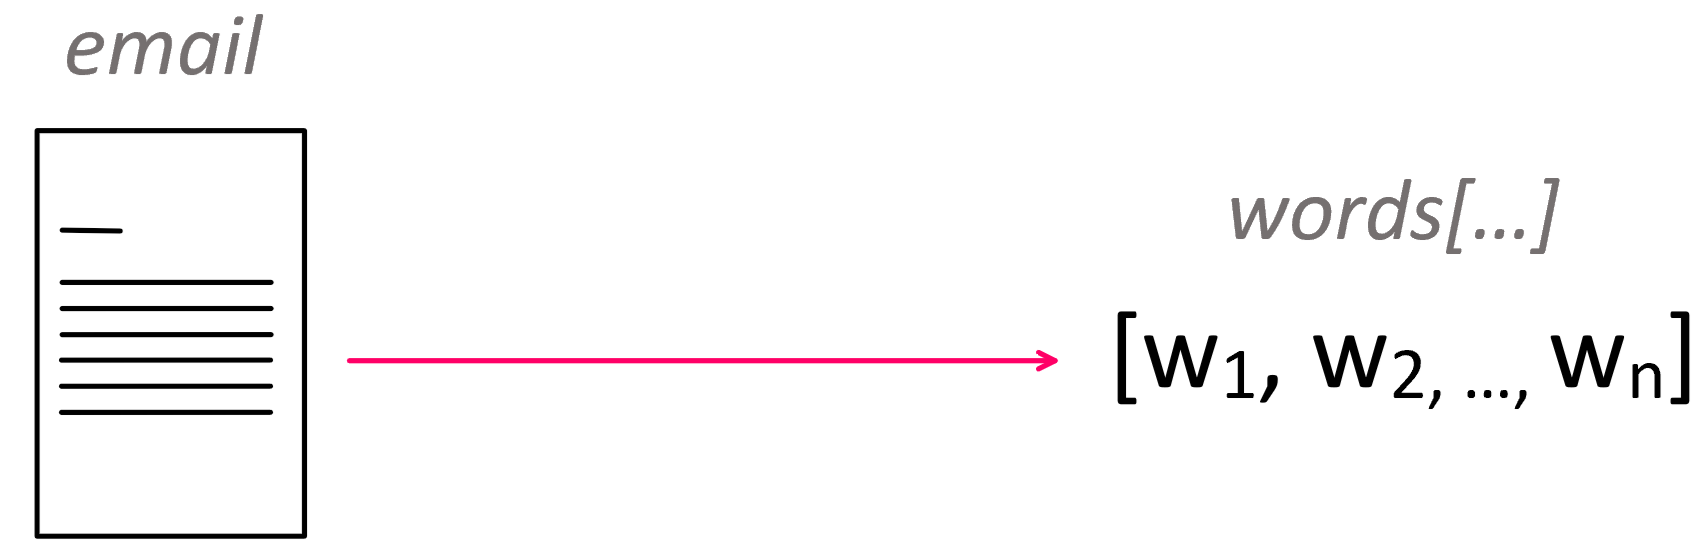
\includegraphics[width=.6\linewidth]{res/cleaning}
        \caption{Cleaning one email resulting into an array of words}
        \label{fig:cleaning}
    \end{figure}

    \item Filtering

    The remaining words may be meaningful now, but most of them may not be 
    relevant. So the next operation will perform an intersection between the 
    words and a list of predefined relevant words. All the words that reside 
    in both lists will remain, but unlike sets, the list contains duplicates.
    As the last filtering step, the words are counted, and a corpus is created.

    \begin{figure}[ht!]
        \centering
        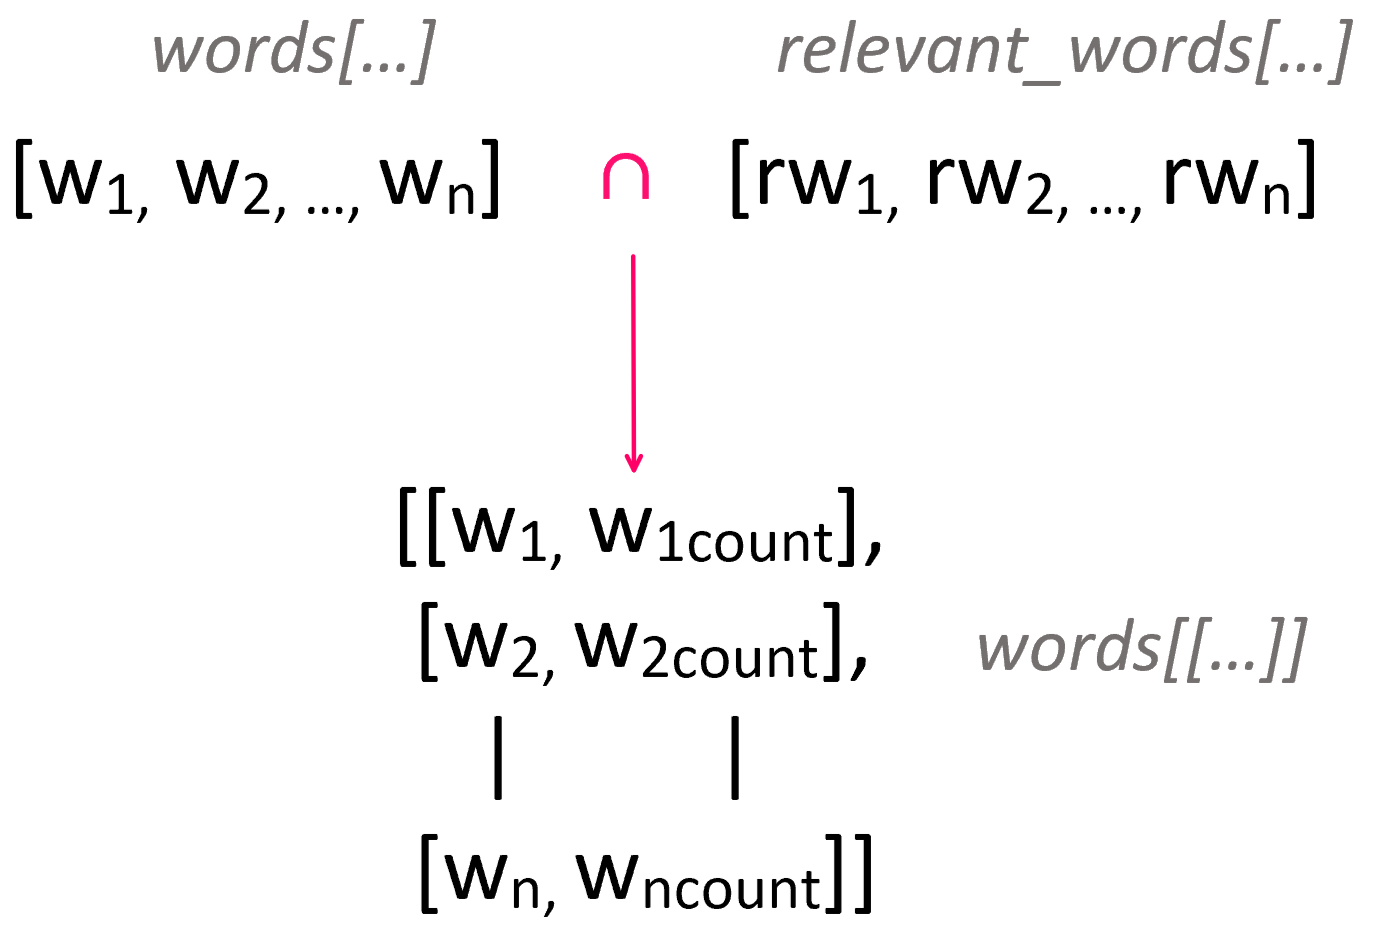
\includegraphics[width=.6\linewidth]{res/filtering}
        \caption{Taking the intersection of the words with a relevant list of words}
        \label{fig:filtering}
    \end{figure}

    \item Ranking

    Other predefined sets of words within the set of relevant words share the 
    same characteristics. For example a set $T \subseteq R$ exists where $T$ 
    is the set of technical words, and $R$ is the set of relevant words from 
    before. Feature list of technical words: $T = [t_1, t_2, \dots, t_n]$. 
    Other feature lists contain other themed words: $U$, $V$, $W$.

    For every word in the email that is present in $T$, a score is calculated 
    that takes the count of that word into account in relation to the total 
    number of relevant words in the email. This calculation is made for all 
    feature lists ($T$, $U$, $V$, $W$), for every word in the email.

    \begin{figure}[ht!]
        \centering
        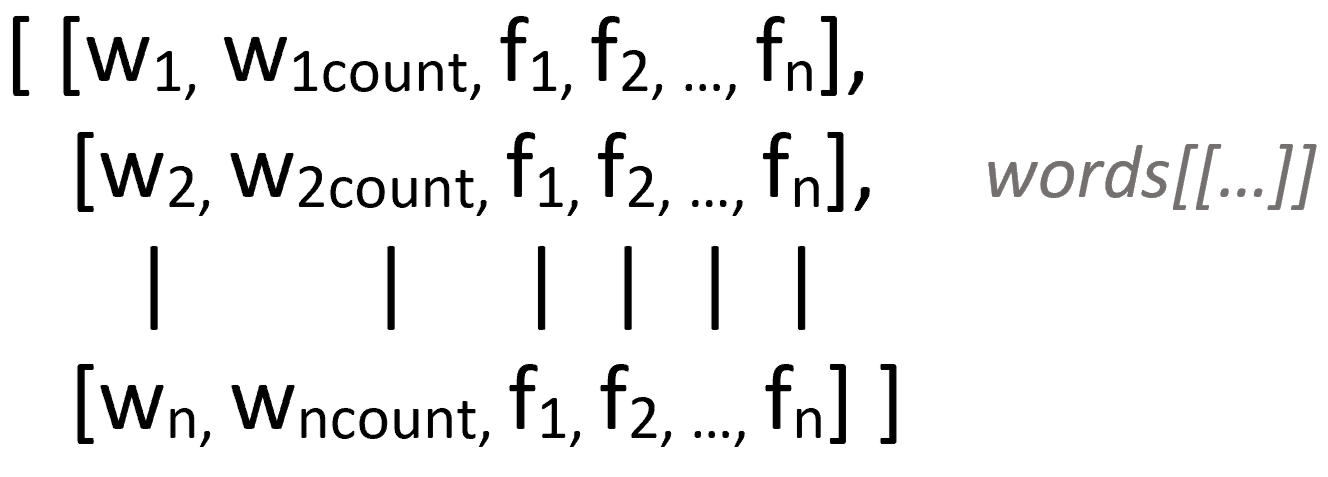
\includegraphics[width=.6\linewidth]{res/ranking}
        \caption{The scores for each words are added as features}
        \label{fig:ranking}
    \end{figure}

    \item Classifying

    Finally the scores are aggregated, resulting in the inputs for the FLS, 
    which outputs the correct department.

    \begin{figure}[ht!]
        \centering
        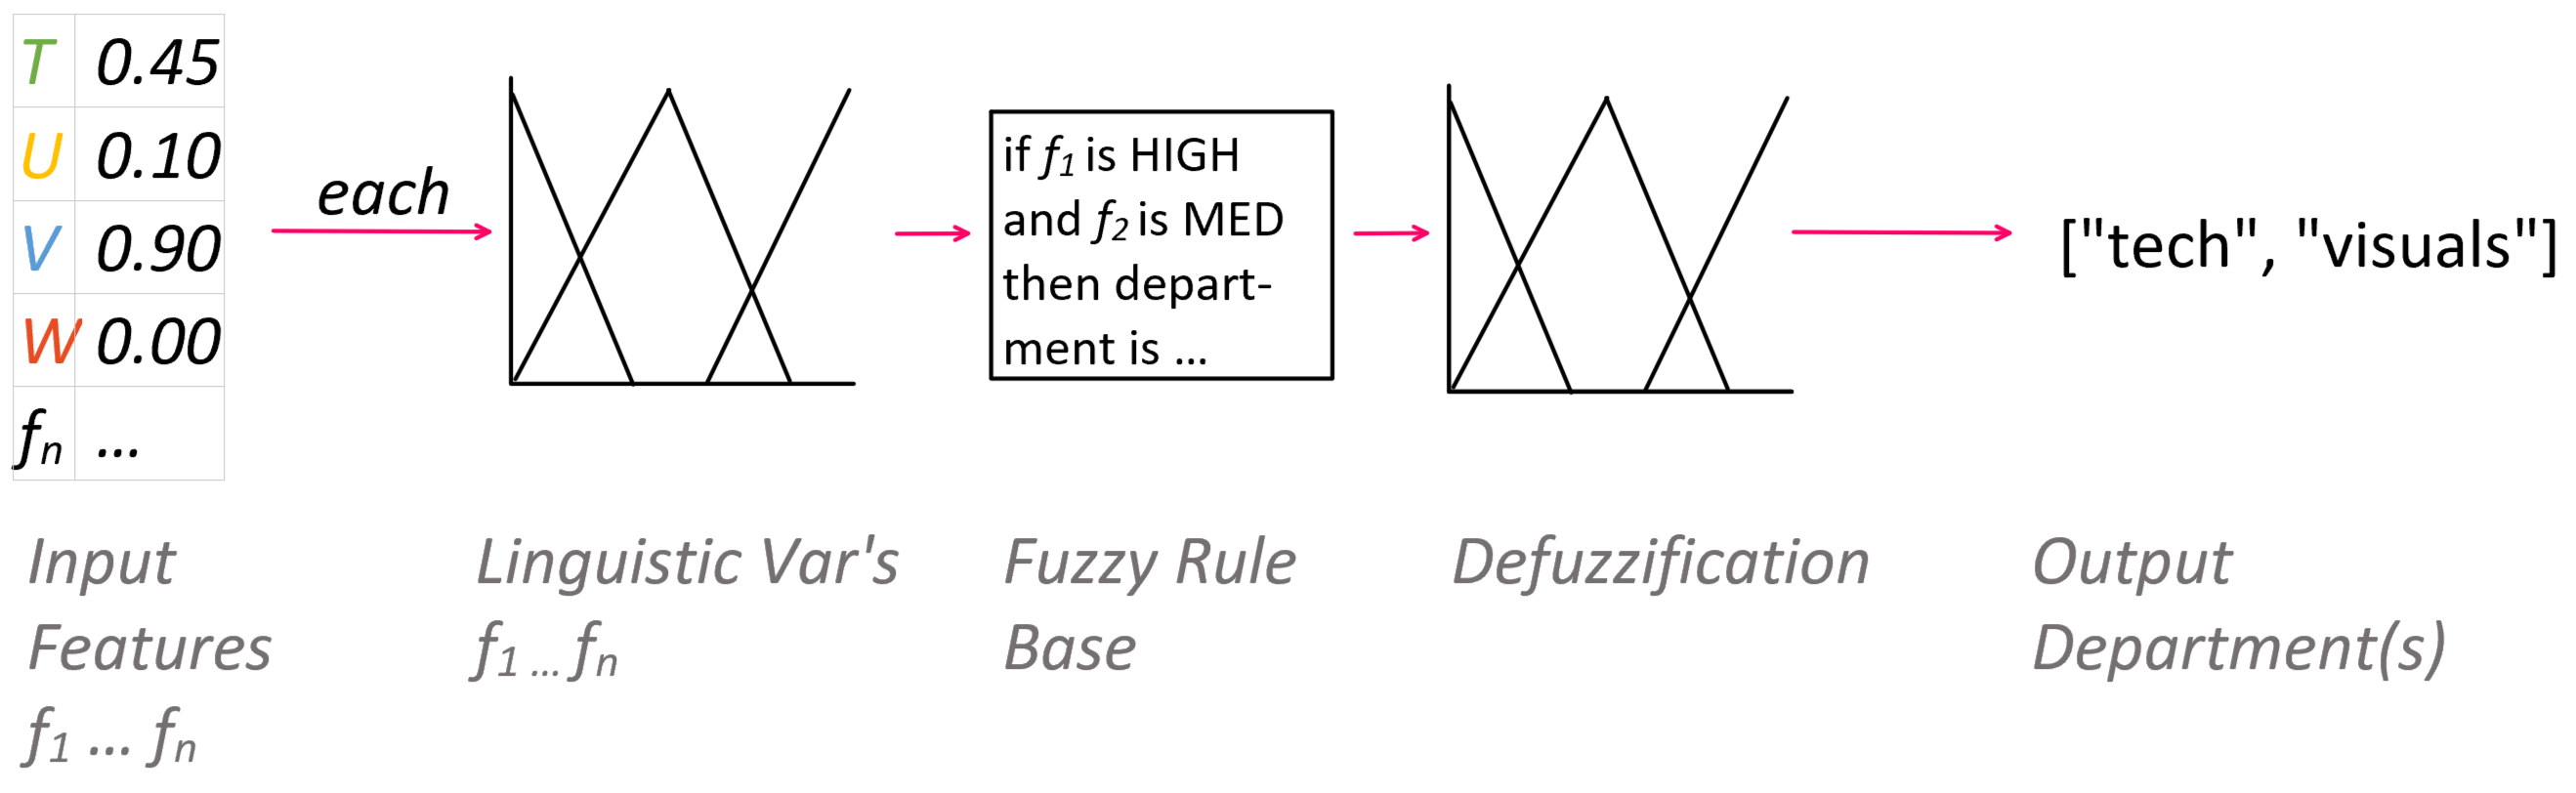
\includegraphics[width=.9\linewidth]{res/classifying}
        \caption{The FLS outputs the department based on the input features}
        \label{fig:classifying}
    \end{figure}
    
\end{enumerate}


\subsection{Implementation}
We used Python3 as programming language and Jupyter Notebook as development 
environment. The four steps mentioned in subsection \ref{subsec:design} are 
roughly coded as follows:

\begin{lstlisting}
// Cleaning
emails = get_emails_from_dataset()

for each email in emails
  tokenize(email)
  lowercase(email)
  remove_punctuation(email)
  keep_only_words(email)
  remove_stopwords(email)
  stem_words(email)

// Filtering
  relevant_words = get_relevant_words()
  corpus = intersection(email, relevant_words)
  corpus = count_wordfrequencies(corpus)
	
// Ranking
  feature_set = get_feature_set()
	
  for each word in corpus:
    for each feature in feature_set:
	  word = calculate_score(word, feature)

// Classifying
  email_score = aggregate_scores(corpus)
	
  FLS = get_fuzy_logic_system()
  department = FLS.calculate_department(email_score)
  send_original_email_to(department)
\end{lstlisting}


% trigger a \newpage just before the given reference
% number - used to balance the columns on the last page
% adjust value as needed - may need to be readjusted if
% the document is modified later
%\IEEEtriggeratref{8}
% The "triggered" command can be changed if desired:
%\IEEEtriggercmd{\enlargethispage{-5in}}

\begin{thebibliography}{9}
\bibitem{email_statistics}
    The Radicati Group, inc.,
    \textit{
        \href{https://github.com/Menziess/Fuzzy-Logic-Email-Classification/raw/master/report/res/a_new_fuzzy_logic_based_ranking_function_for_efficient_information_retrieval_system.pdf}{Email Statistics Report, 2015-2019},
    }
    accessed: Nov 28, 2017.

\bibitem{spam}
    G.Santhi, S. Maria Wenish, Dr. P. Sengutuvan,
    \textit{
        \href{https://github.com/Menziess/Fuzzy-Logic-Email-Classification/raw/master/report/res/a_content_based_classification_of_spam_mails_with_fuzzy_word_ranking.pdf}{A Content Based Classification of Spam Mails with Fuzzy Word Ranking},
    }
    Department of Information Science and Technology,
    Issue 3,
    2013.

\bibitem{phishing}
    Rosana J. Ferolin,
    \textit{
        \href{https://github.com/Menziess/Fuzzy-Logic-Email-Classification/raw/master/report/res/a_proactive_anti-phishing_tool_using_fuzzy_logic_and_ripper_data_mining_classification_algorithm.pdf}{A Proactive Anti-Phishing Tool Using Fuzzy Logic and RIPPER Data Mining Classification Algorithm},
    }
    Department of Computer Engineering University of San Carlos.

\bibitem{ranking}
    Rosana J. Ferolin,
    \textit{
        \href{https://github.com/Menziess/Fuzzy-Logic-Email-Classification/raw/master/report/res/a_new_fuzzy_logic_based_ranking_function_for_efficient_information_retrieval_system.pdf}{A new fuzzy logic based ranking function for efficient Information Retrieval system},
    }
    Department of Electrical Engineering Dayalbagh Educational Institute,
    2014.

\end{thebibliography}

\end{document}


